\chapter{Nuclear Models}

\section{Introduction}

In the following, it is worth to make a discussion about the nuclear models that are used by theoreticians in order to describe phenomena that are specific to rotating nuclei and high-spin regime. Since the focus of this work emerges from a \emph{class} of properties that usually apply to the high-spin region (but this does not necessarily also imply a high-energy region), it makes sense to give an insight in the tools that fit the best the underlying effects.

\section{Shell model}

The fact that an atomic nucleus can have a structure that behaves rather similarly as its \emph{parent} (i.e., the atom) in terms of changing the number of constituents, has been enforced by the experimental observations that were done across time. The sharp and discrete discontinuities of nuclear properties, such as the nucleon separation energy, point to the fact that nucleus can be explained through the existence of \emph{shells}. Some examples of observations which indicate this are:
\begin{itemize}
    \item When adding a nucleon to a nucleus, there are certain places where the \emph{binding energy} of the next nucleon becomes considerably smaller than the previous one. 
    \item Separation energies for both the protons and neutrons suffer drastic changes, having strong deviations from the predictions of the semi-empirical mass formula \cite{weizsacker1935theorie}, the discontinuities being represented by major shell closures (complete filling) \cite{krane1991introductory}.
    \item The neutron absorption cross-section has a substantial decrease in value at the neutron magic numbers
    \item Great abundance of nuclides where $Z$ and $N$ are magic numbers.
\end{itemize}

The sudden discontinuities occur at specific values of the proton $Z$ and neutron $N$ numbers: these are called \emph{magic numbers}. Currently, these magic numbers correspond to $Z$ or $N=2,8,20,28,50,82,126$, and they represent the so-called major shells. There are also two \emph{weakly magic numbers}: 40 and 64.

One can examine the values for the first excited states $2^+$ that are shown in Figs. \ref{e2plus_proton}, \ref{e2plus_neutron}. Indeed, these values show some peaks, each peak corresponding to a particular magic number.

\begin{figure}
    \centering
    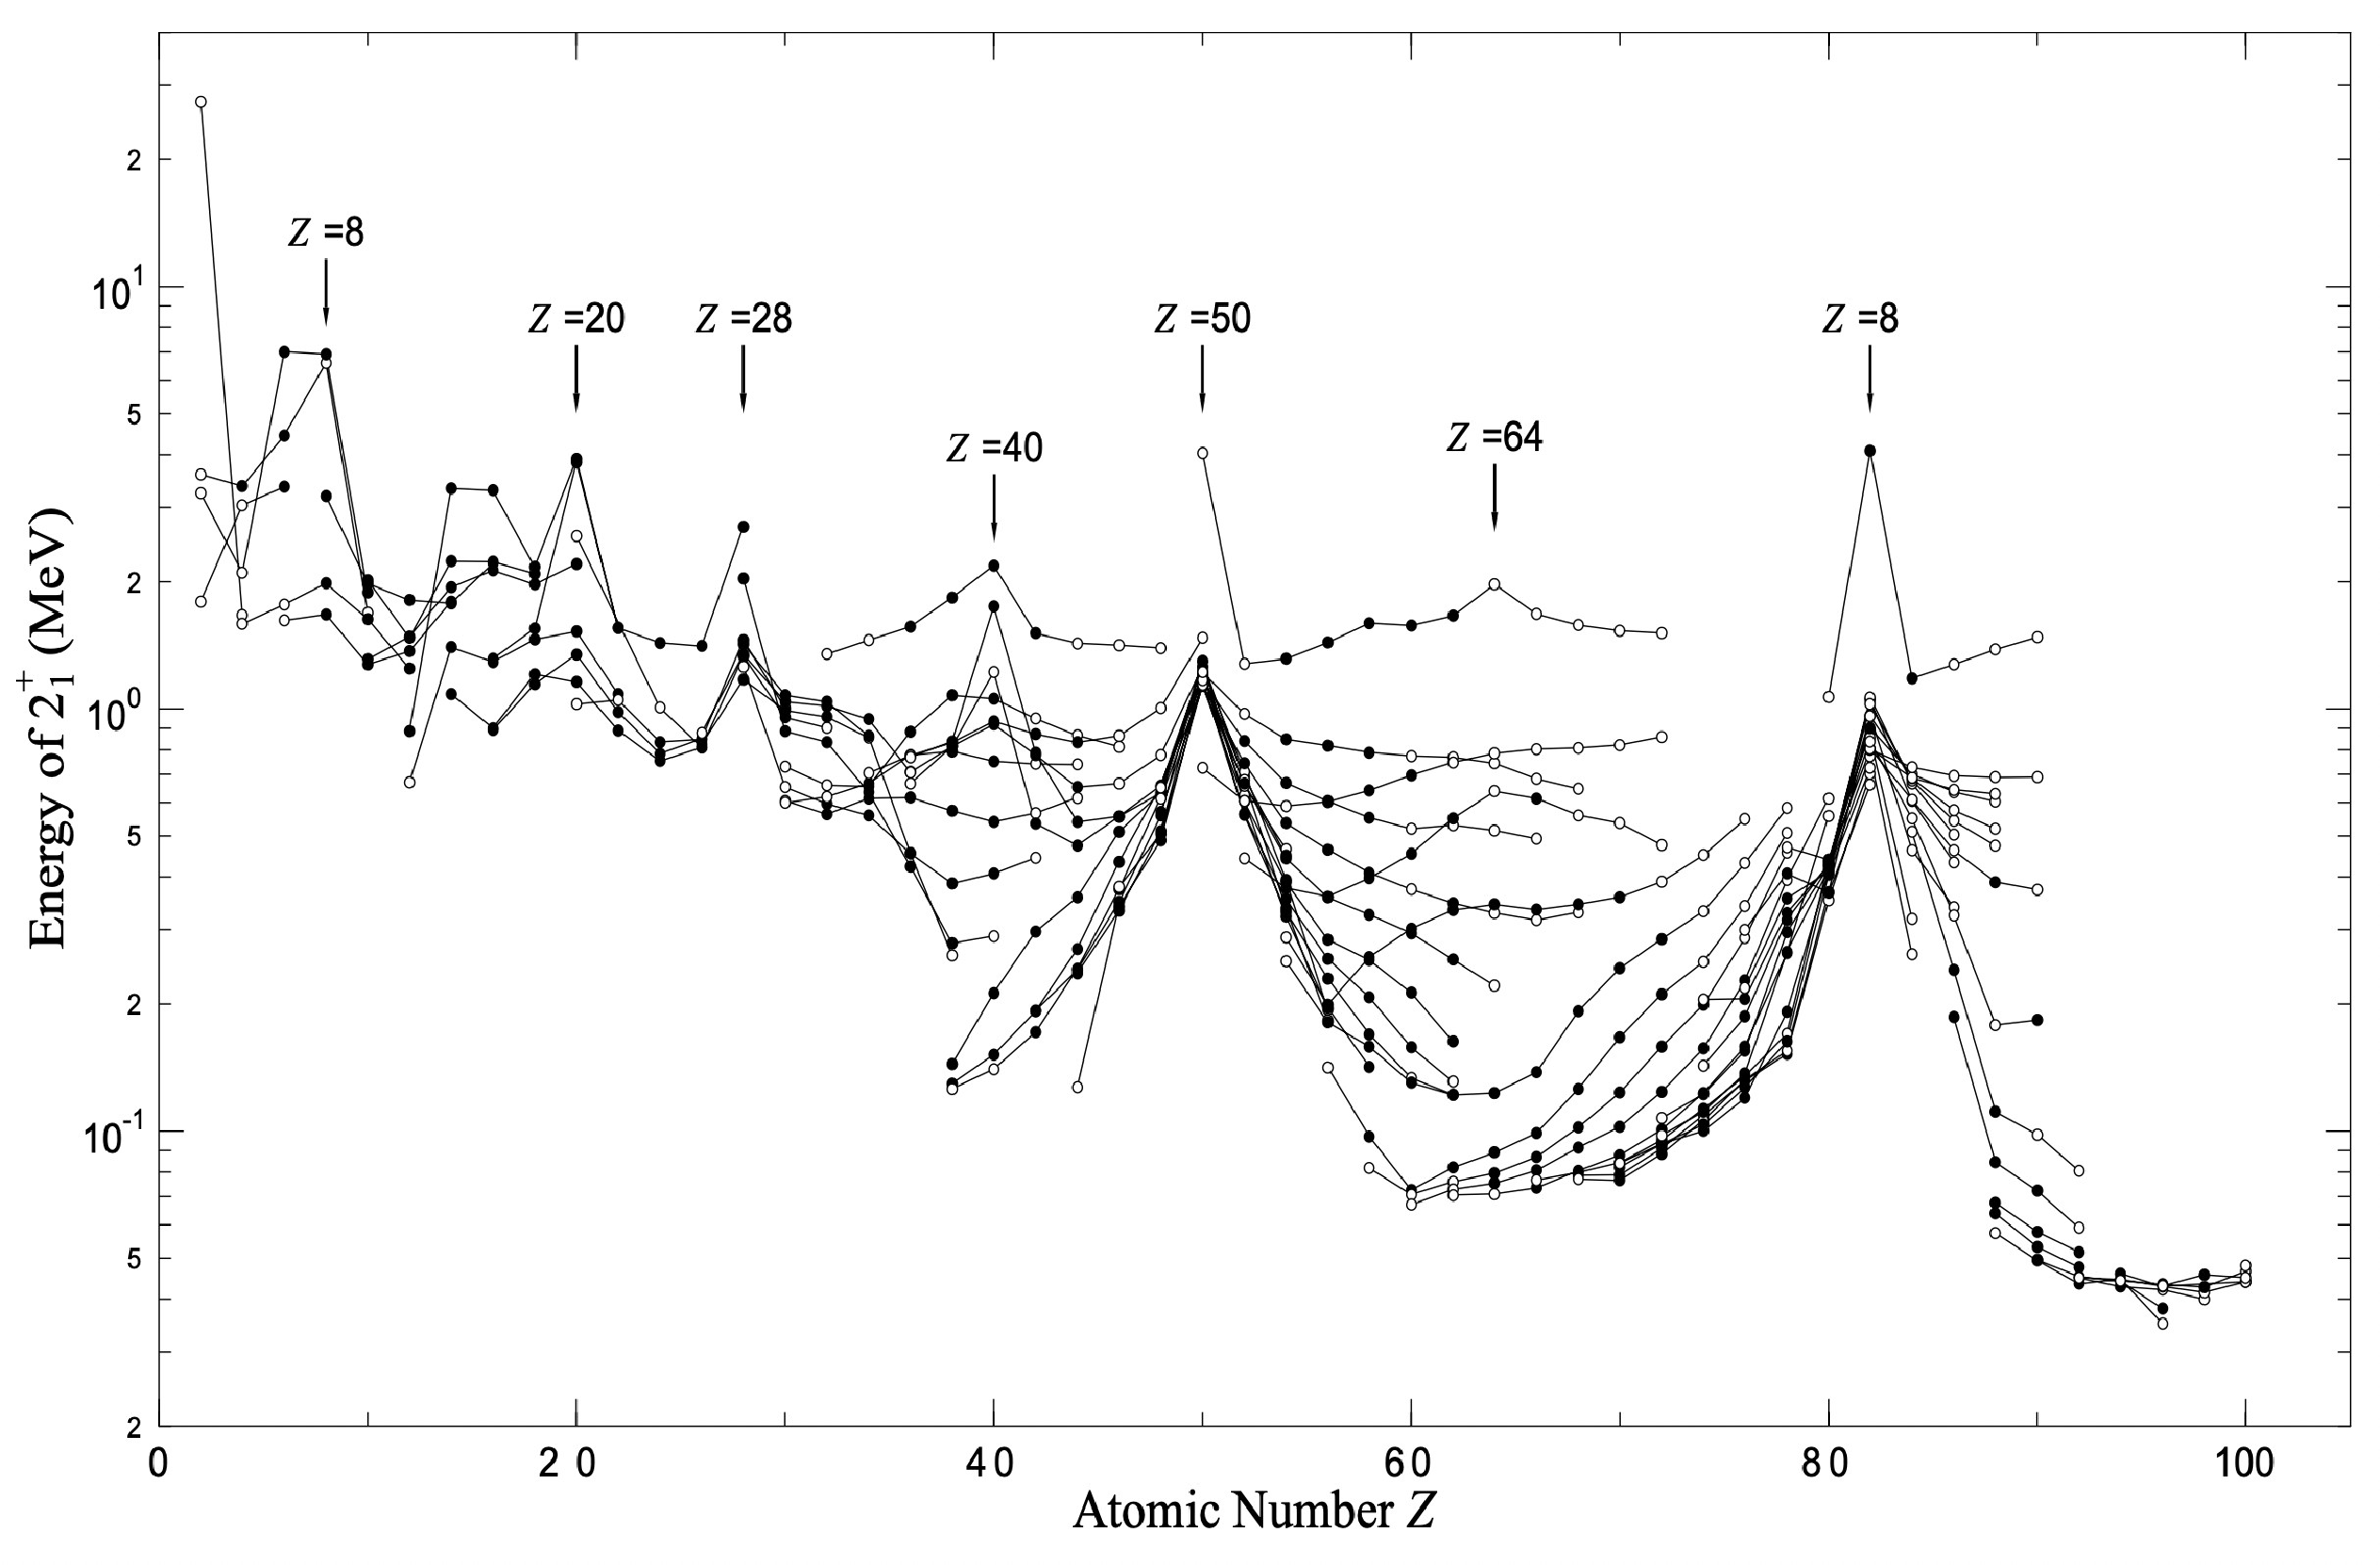
\includegraphics[scale=0.33]{Chapters/Figures/E2plus_proton.pdf}
    \caption{The first excited energy states $2^+$ of nuclei with even $Z$ and $N$ graphically represented with respect to the proton number. Each line represents a set of isotopes. Figure taken from Ref. \cite{matta2017exotic}.}
    \label{e2plus_proton}
\end{figure}

\begin{figure}
    \centering
    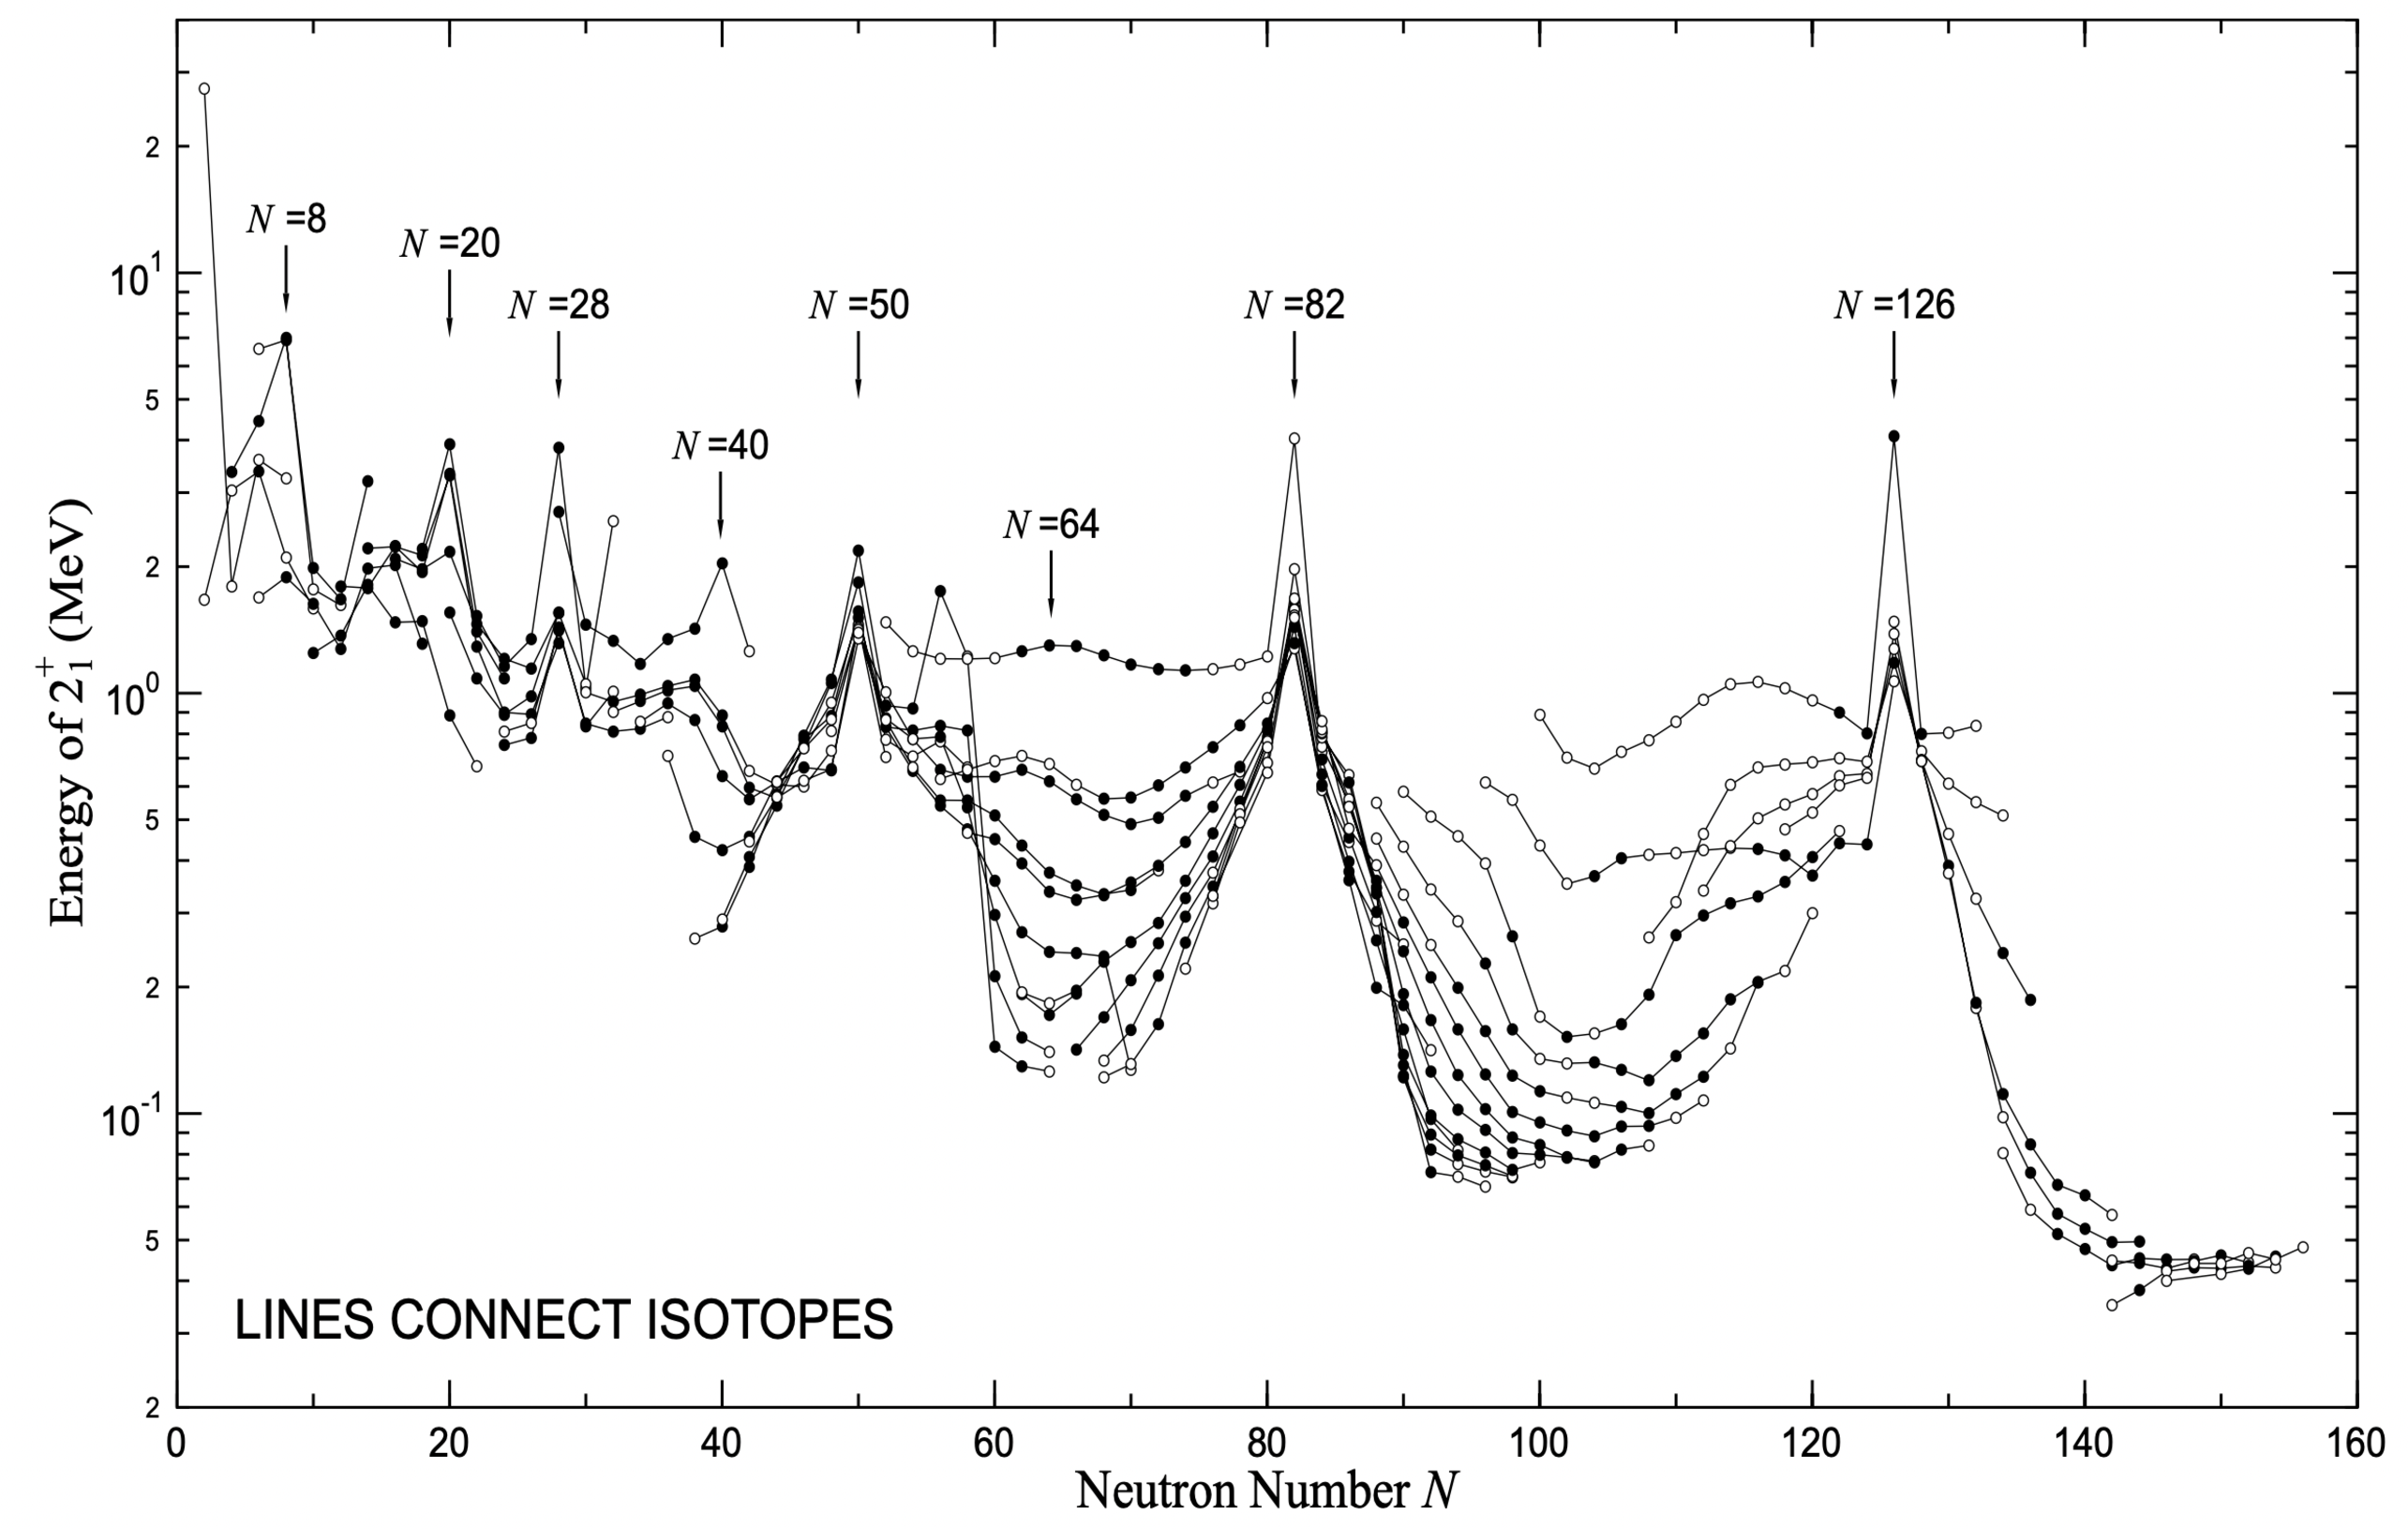
\includegraphics[scale=0.33]{Chapters/Figures/E2plus_neutron.pdf}
    \caption{The first excited energy states $2^+$ of nuclei with even $Z$ and $N$ graphically represented with respect to the neutron number. Each line represents a set of isotopes. Figure taken from Ref. \cite{matta2017exotic}.}
    \label{e2plus_neutron}
\end{figure}

The shell model starts from the basic assumption that the nucleus is a \emph{mean-field potential}, that is a potential for which the motion of a single nucleon is caused by all the other nucleons (the nucleon is moving inside an average potential generated by all the other constituents of the nucleus). Of course, all the nucleons that are under the influence of such a mean field potential occupy the energy levels which correspond to a series of (sub)shells that agree with the Paul exclusion principle. Having a general expression for the potential that properly reproduces all the magic numbers (and the observed nuclear properties) is the main goal.

Since the model starts from the concept of independent (non-interacting) particle motion within an average potential, finding each energy will be equivalent of solving the Schrödinger equation:
\begin{align}
    -\frac{\hbar^2}{2m}\nabla ^2\psi_i(r)+V(r)\psi_i(r)=e_i\psi_i(r)\, 
    \label{schrodinger-single-particle-eq}
\end{align}
where $e_i$ represents the energy (eigenvalue) and $\psi_i$ represents the wave-function (eigenstates), while $V(r)$ is the nuclear potential whose expression must be evaluated.

The choice of $V(r)$ will be dictated by the reproduction of various experimental data (such as nuclear saturation, scattering, nuclear reactions, and so on). For the motion of an independent particle, an obvious first attempt would be the \emph{simple harmonic oscillator} (SHO), which has the known expression:
\begin{align}
    V(r)=\frac{1}{2}m(\omega_i r)^2\ ,
    \label{harmonic-potential}
\end{align}
with $\omega_i$ as the frequency of the basic harmonic-like motion of the particle in the nucleus. With Eq. \ref{harmonic-potential}, the motion of the nucleon has a straightforward expression:
\begin{align}
    \frac{\hbar^2}{2m}\nabla^2\psi_i(r)+\frac{1}{2}m(\omega r)^2\psi_i(r)=e_i\psi_i(r)\ .
\end{align}

This Schrödinger equation has its energy eigenvalues under to form:
\begin{align}
    e_N=\left(N+\frac{3}{2}\right)\hbar\omega\ ,
\end{align}
where $N$ is the number of oscillator quanta which describes each major shell (also called the \emph{principal quantum number}). One should keep in mind that such an expression is typical for a three-dimensional and isotropic harmonic oscillator. The principal quantum number $N$ is furthermore defined as:
\begin{align}
    N=2(n-1)+l\ ,
\end{align}
with $n$ and $l$ being the \emph{radial} quantum number and \emph{orbital angular momentum} quantum number, respectively, taking values $n=1,2,3,\dots$ and $l=0,1,2,\dots,n-1$. In this first approximation, all the levels with the same principal quantum number $N$ are \emph{degenerate}, with a maximal degeneracy given by $2(2l+1)$. However, by using only the SHO term as the expression of $V(r)$, only the first three magic numbers are reproduced, meaning that some additional term(s) might be needed in order to consistently obtain the series of magic numbers.

A next step is to use the fact that the experimentally observed short range of the strong nuclear force: the steepness of the SHO can be corrected with an \emph{attractive} term proportional to $l$-squared. This acts as a centrifugal term which provides an angular momentum barrier, lifting the degeneracy between the levels with the same principal quantum number $N$ and different values for the orbital angular momentum $l$. This SHO+$l^2$ step is still not enough though. The last step is to add a so-called \emph{spin-orbit} coupling term of the form $\vec{l}\cdot\vec{s}$. 
% This last term is enough to reproduce all the magic numbers and the experimentally measured quantities that are relevant to the shell model itself.
This term comes from the consideration that the nucleon-nucleon interaction has a spin dependence, and the potential depends on the intrinsic spin $s$ ($\vec{s}$) and the orbital angular momentum $l$ ($\vec{l}$) of a nucleon. Since $\vec{j}=\vec{l}+\vec{s}$, two possible states emerge from a single value of $l$ (depending on wether $\vec{s}$ is parallel or anti-parallel to $\vec{l}$). The final expression of the terms SHO+$\vec{l}^2$+$\vec{l}\cdot\vec{s}$ will consist in the \emph{Modified Harmonic Oscillator} (HMO).
\begin{align}
    V(r)=\frac{1}{2}(\omega r)^2+B\ \vec{l}^2+A\ \vec{l}\cdot\vec{s}\ .
    \label{modified-harmonic-oscillator-eq}
\end{align}

For the sake of simplicity, the centrifugal term will be denoted within formulas without the vector symbol. Since the intrinsic spin of a nucleon is $s=1/2$, for a given value of $l$, there can be two values for the \emph{total angular momentum} (a.m.) $j=l\pm1/2$: one for each spin orientation with respect to the direction of the orbital a.m. Moreover, for each value of $l=0,1,2,3,4,\dots$, there is a similar notation $l=s,p,d,f,g,\dots$, respectively. Regarding the spectroscopic notation, usually, the value of $j$ is considered as a subscript; $nl_j$ (for example $1p_{1/2}$ and $1p_{3/2}$). What it is worth mentioning is that for high enough shells, there can be splittings between $j+1/2$ and $j-1/2$ that are large enough to lower the $j+1/2$ state from one oscillator shell $n$ to one located below $n-1$. These types of levels are called \emph{intruder states} and they have opposite parity $\pi=(-1)^l$ with respect to the shell that these levels will occupy.

Going back to the expression of the $\vec{l}\cdot\vec{s}$ term from Eq. \ref{modified-harmonic-oscillator-eq} and denoting it with $V_{ls}(r)$, it is shown by Casten \cite{casten2000nuclear} that its contribution to the total potential can be regarded as a surface effect. Due to this, its form can be expressed as a function that depends on the radial coordinate as such \cite{casten2000nuclear}:
\begin{align}
    V_{ls}(r)=-a_{ls}\frac{\partial V(r)}{\partial r}\vec{l}\cdot\vec{s}\ ,
\end{align}
where $V(r)$ is the expression for a central potential and $a_{ls}$ is a strength constant.
% Indeed, in the work of Casten \cite{casten2000nuclear}, it is stated that if in the nucleus, the spin-orbit forces were large enough, then there should be an overall preference for nucleons with spins aligned parallel their orbital a.m. other than the opposite alignment, making the nucleons with anti-parallel spins to not be surrounded by an equal number of nucleons with all spin orientations.

Now that an expression for the nuclear potential that is able to reproduce all the magic numbers has been formulated, it is also possible to formulate the total energy of a single-particle within the average potential that is generated by all the other nucleons within the nucleus. Thus, the Hamiltonian of this simple system (the modified oscillator) can be formulated as such:
\begin{align}
    H&=-\frac{\hbar^2}{2m}\nabla^2+V_\text{SHO}+(l^2)_\text{term}+(\vec{l}\cdot\vec{s})_\text{term}=-\frac{\hbar^2}{2m}\nabla^2+V_\text{MHO} , \nonumber\\
    H&=-\frac{\hbar^2}{2m}\nabla^2+\frac{1}{2}m(\omega r)^2+Bl^2+A\vec{l}\cdot\vec{s}\ .
\end{align}

The evolution from each term in the shell-model potential (that is the first approximation as a SHO, then SHO+$l^2$, and finally SHO+$l^2+\vec{l}\cdot\vec{s}$ or modified oscillator potential) is illustrated in Fig. \ref{energy-levels-mho}, where it can be seen how each extra term introduces a new degeneracy within the energy states, with the complete reproduction of the magic numbers in the third column. Moreover, the \emph{intruder} levels can be observed, where levels with $j=l+1/2$ from a particular $n$ are so low, that they lie below an $n-1$ adjacent level.
\begin{figure}
    \centering
    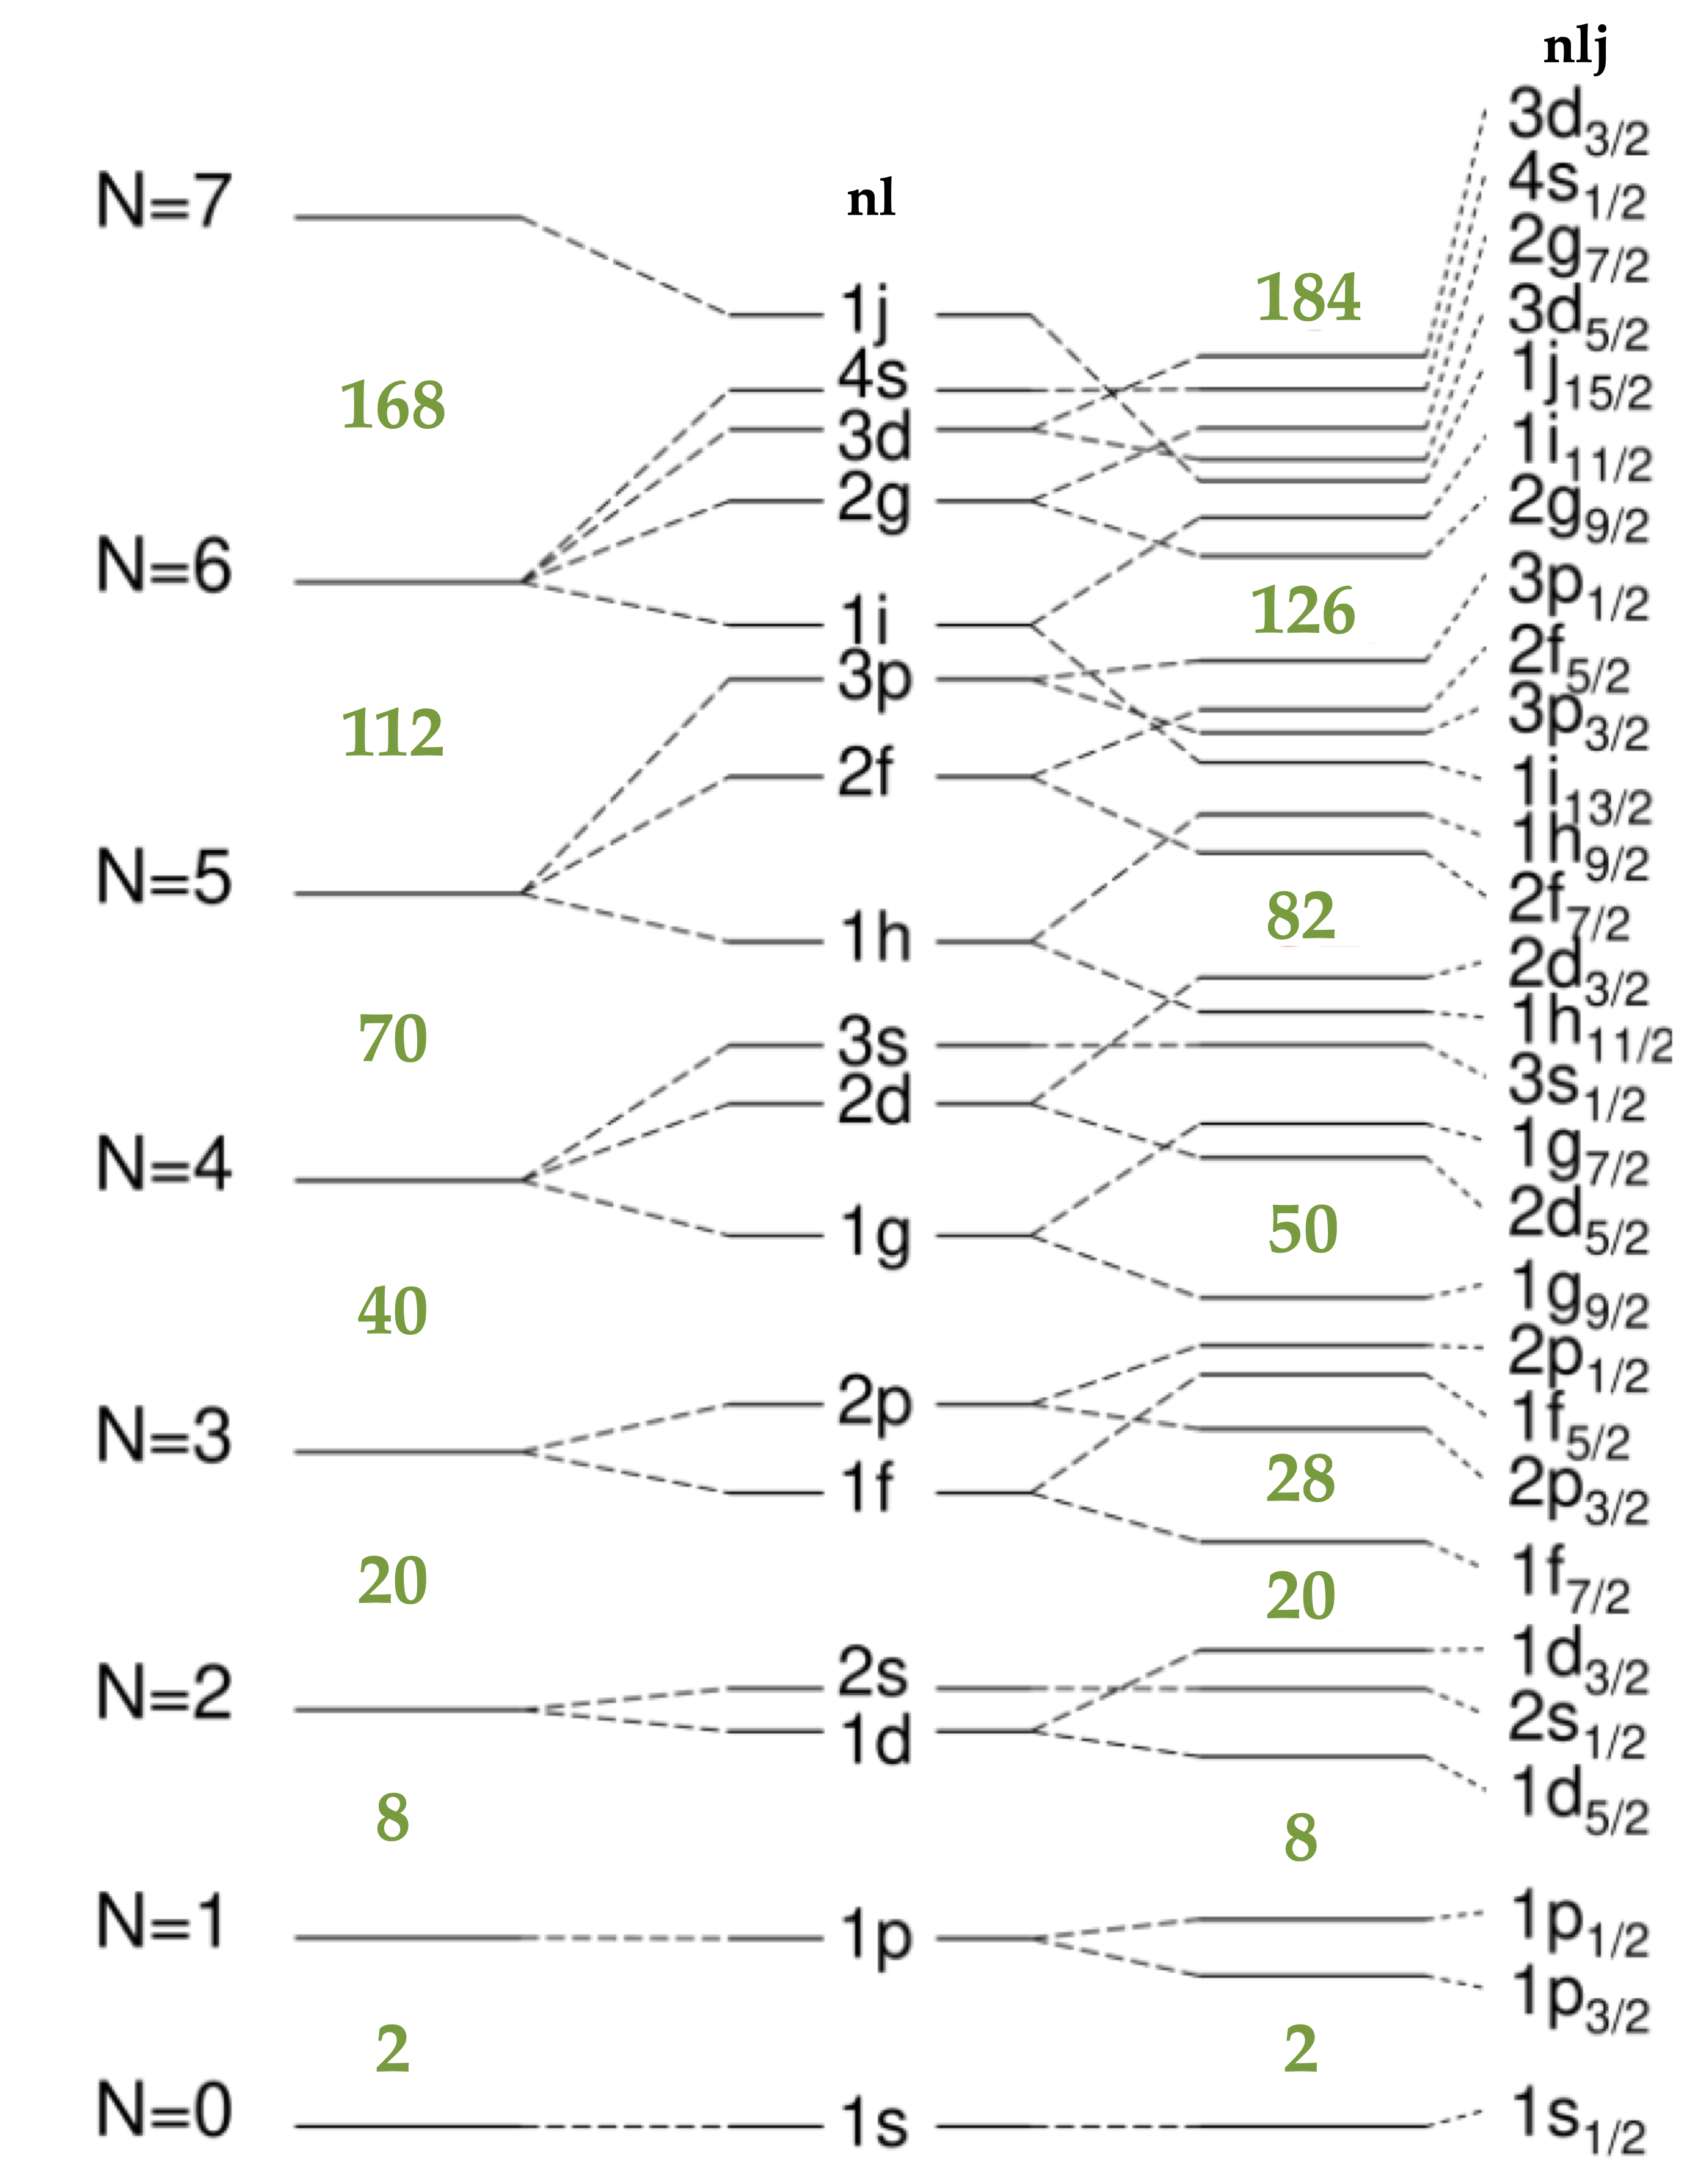
\includegraphics[scale=0.12]{Chapters/Figures/SM_level_scheme.png}
    \caption{The energy levels obtained via calculation of the shell model potential using the simple oscillator (SHO), the SHO amended with a centrifugal term $l^2$, and finally the modified oscillator (MHO) that contains a spin-orbit term. The `correct' magic numbers are the ones in the right-most column. Figure is adapted from Refs. \cite{matta2017exotic},\cite{krane1991introductory}.}
    \label{energy-levels-mho}
\end{figure}

Another, more realistic potential that can be used in order to reproduce the specific shell model calculation is the so-called Woods-Saxon potential. Because of the short-range character of the strong nuclear force, it is safe to assume that this potential should behave in the same manner as the density distribution of the nucleons. Since for medium and heavy nuclei, the Fermi-like functions (distributions) are the ones that best fit the experimentally measured data, this potential should have the following form \cite{woods1954diffuse}:
\begin{align}
    V_\text{ws}(r)=-\frac{V_0}{1+e^{\frac{r-R_0}{a}}}\ .
    \label{woods-saxon-potential}
\end{align}
This mean-field potential contains the terms $V_0$ that represents the depth of the potential ($\approx 50$ MeV, in order to reproduce the experimental separation energies for the nucleons), the surface thickness $a$ (also called the diffuseness parameter, giving information about how fast the potential drops to zero) with a value of approximately $0.5$ fm, while $R_0$ is the nuclear radius with $R_0=r_0A^{1/3}$ and $r_0=1.2$ fm. The nature of this potential is of \emph{central type} and, unfortunately, Eq. \ref{woods-saxon-potential} in its pure form is not enough the reproduce the higher magic numbers. As such, the addition of a spin-orbit term, similarly as in the case of MHO potential, is required \cite{martin2017particle}: 
\begin{align}
    V_\text{total}=V_\text{ws}^\text{central}+V_{ls}(r)\vec{l}\cdot\vec{s}\ .
    \label{woods-saxon-so-potential}
\end{align}
The only good quantum numbers in the case of the WS potential are the total a.m. $j$ and the parity $\pi=(-1)^l$.
The expectation value of the spin-orbit term $\vec{l}\cdot\vec{s}$ can be given as:
\begin{align}
    \langle ls \rangle=\hbar^2\begin{cases}
        \frac{l}{2} \quad &\text{for} j=l+\frac{1}{2}\\
        -\frac{l+1}{2} &\text{for} j=l-\frac{1}{2}\ \\
   \end{cases}\ .
\end{align}
and the spacing between two levels can be furthermore expressed as \cite{martin2017particle}:
\begin{align}
    \Delta E_{ls}=\frac{2l+1}{2}\hbar^2\langle V_{ls}\rangle\ .
\end{align}
The experimental evidence points to the fact that $V_{ls}(r)$ is negative, meaning that states with $j=l-1/2$ are shifted higher than $j=l+1/2$. Some characteristics of the WS potential are the following:
\begin{enumerate}
    \item It increases with the increase of $R$, meaning that it has an \emph{attractive nature}
    \item It flattens out for large enough $A$ in the center of the nucleus
    \item It rapidly goes to zero as $R$ increases (given by the diffuseness parameter), indicating its short-range nature
    \item When $R=R_0$ (that is for the nucleons near the surface), a large force towards the center of the nucleus is experienced by the these nucleons.
\end{enumerate}
\begin{figure}
    \centering
    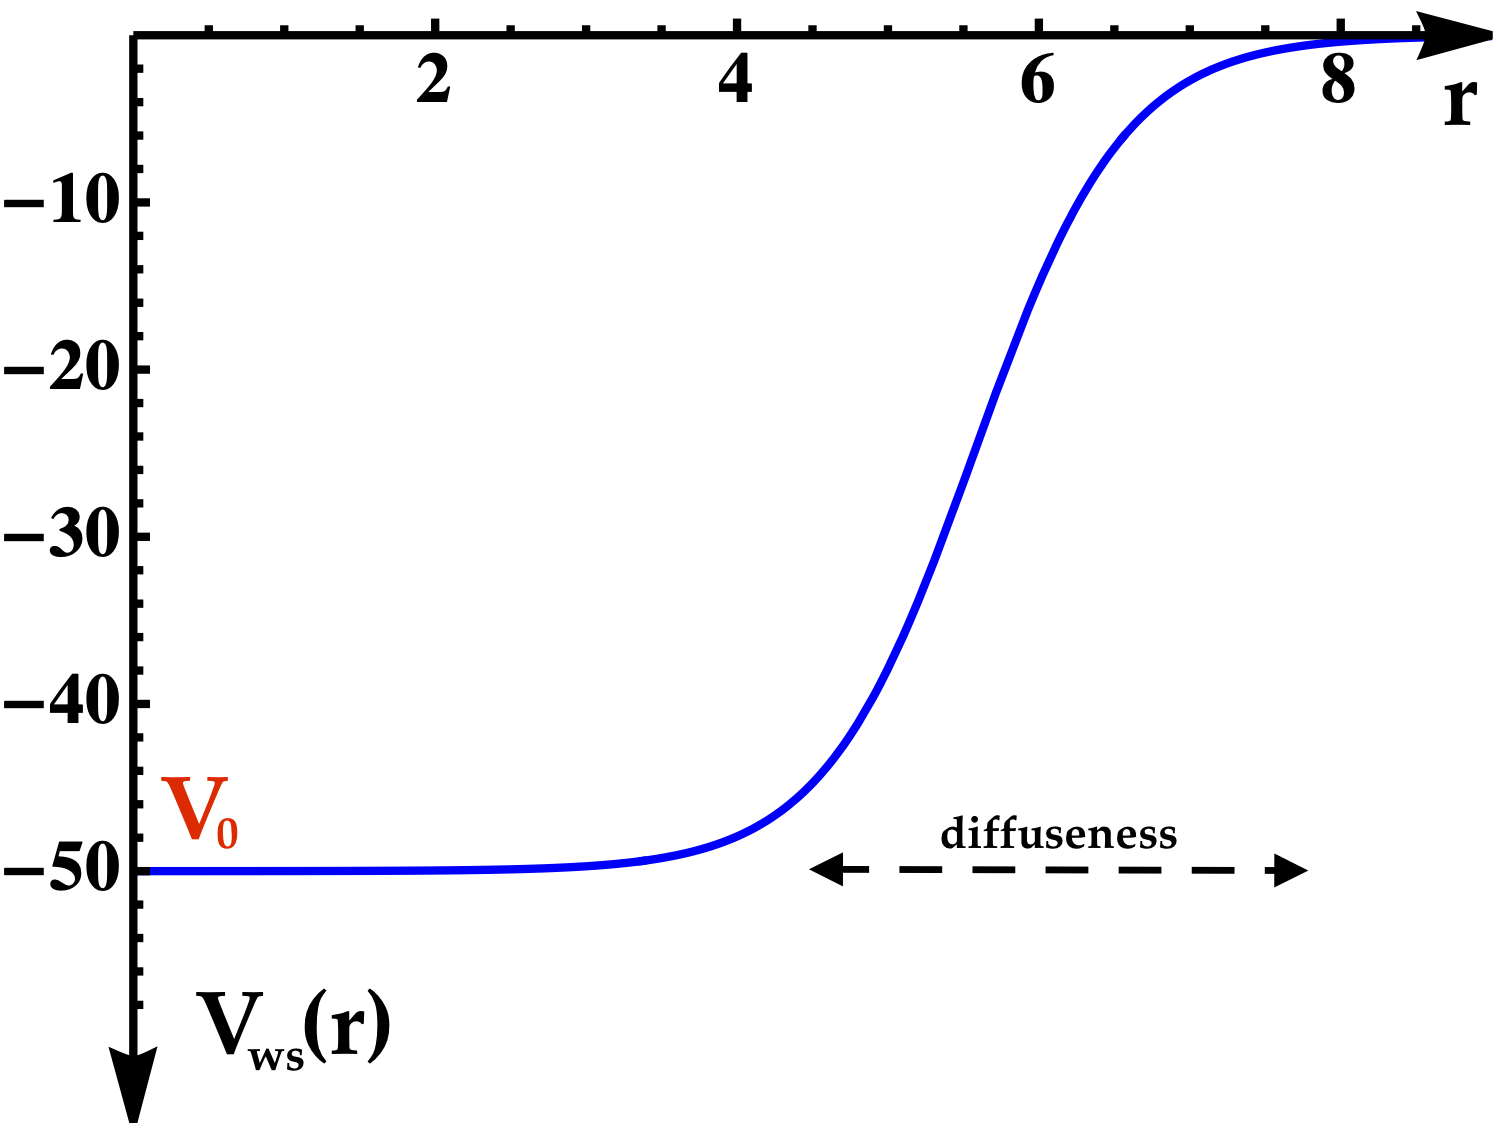
\includegraphics[scale=0.2]{Chapters/Figures/ws_potential_plot.png}
    \caption{The shape of the Woods-Saxon potential, defined by Eq. \ref{woods-saxon-potential}. The parameters are arbitrarily chosen as: $V_0=50$ MeV, $R=5.57$ fm, and $a=0.5$ fm.}
    \label{woods-saxon-plot}
\end{figure}

Fig. \ref{woods-saxon-plot} shows the shape of a typical Woods-Saxon potential. Aiming at a final Hamiltonian which describes the motion of the nucleon within the mean-field potential, the formula can be readily obtained:
\begin{align}
    H&=-\frac{\hbar^2}{2m}\nabla^2+V_\text{ws}^\text{central}+(\vec{l}\cdot\vec{s})_\text{term}\ ,\\
    H&=-\frac{\hbar^2}{2m}\nabla^2-\frac{V_0}{1+e^{\frac{r-R_0}{a}}}+A\vec{l}\cdot\vec{s}\ .
\end{align}
In addition to the shape of the Woods-Saxon potential, a comparison between it, a SHO,and the square-well-like potential is made in Fig \ref{shell-model-functional-potentials}.
\begin{figure}
    \centering
    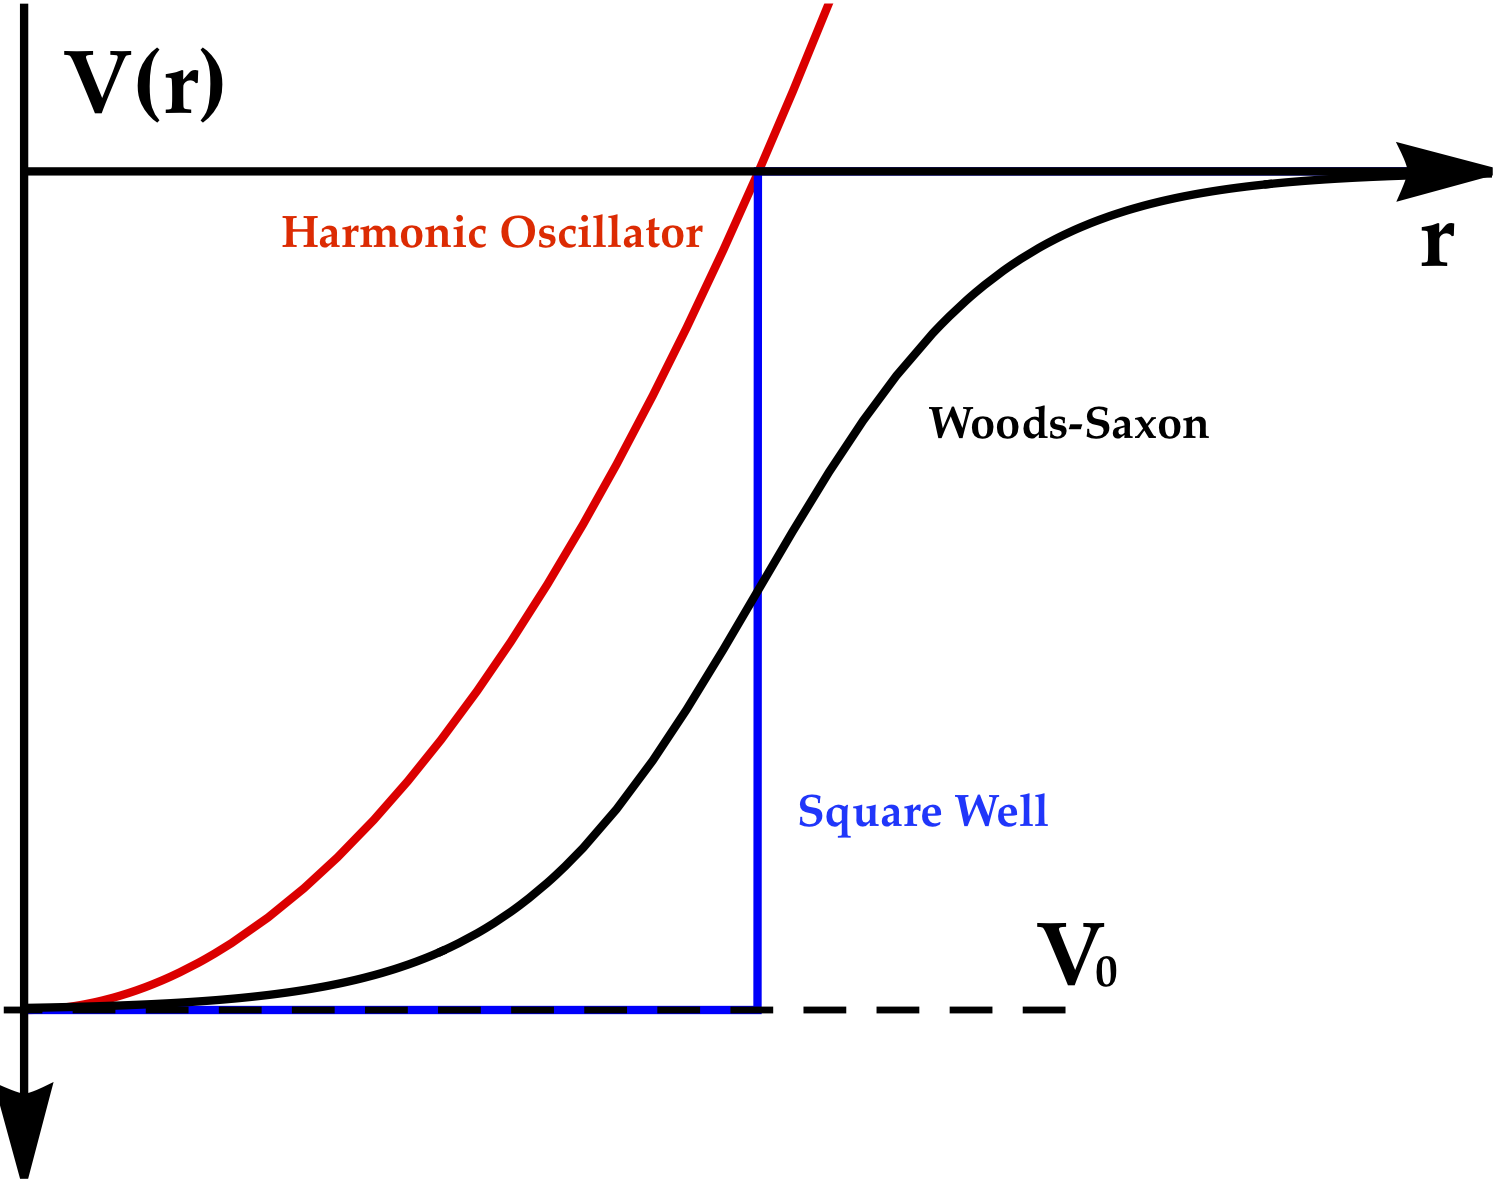
\includegraphics[scale=0.2]{Chapters/Figures/functional-potentials-shell-model.png}
    \caption{A schematic representation with the three kind of potentials used to describe the shell model: harmonic oscillator, Woods-Saxon, and for completeness, the square-well.}
    \label{shell-model-functional-potentials}
\end{figure}

The difference between the pure form of the Woods-Saxon potential and the total potential, where the spin-orbit contribution is amended, can be seen in Fig. \ref{woods-saxon-energy-levels}.
\begin{figure}
    \centering
    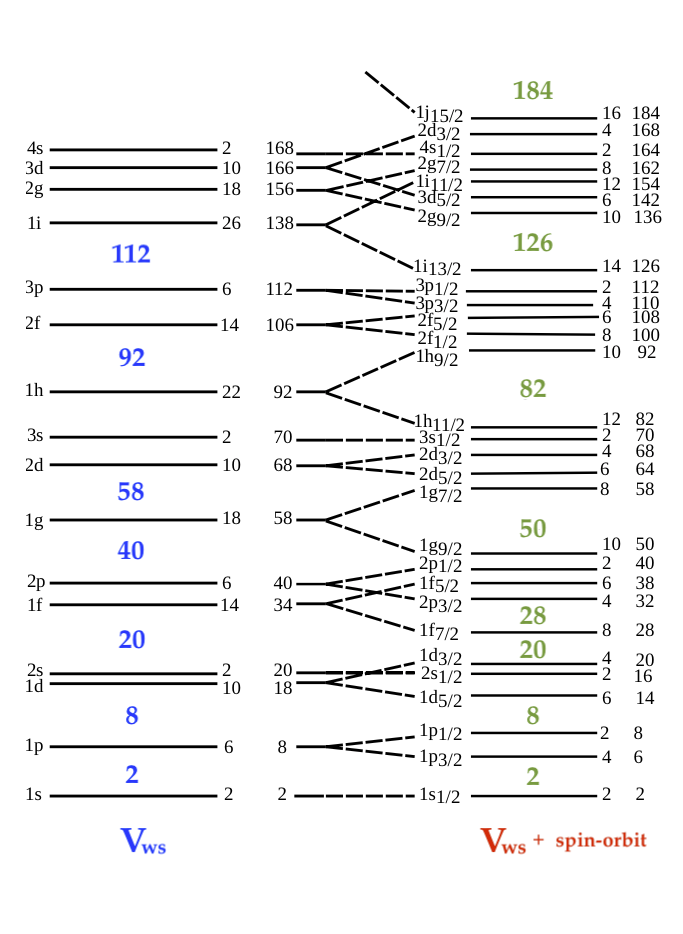
\includegraphics[scale=0.46]{Chapters/Figures/energy_levels_WS.png}
    \caption{The left side represents the energy levels calculated for the Woods-Saxon potential given by Eq. \ref{woods-saxon-potential}, and the right side shows the single-particle energies with the spin-orbit correction added, as in Eq. \ref{woods-saxon-so-potential}. Figure adapted from Ref. \cite{lewis2019lifetime}.}
    \label{woods-saxon-energy-levels}
\end{figure}

So far, the general discussion concerning the nuclear models was for the case where each nucleon is treated as an \emph{independent} particle moving in an average potential (mean-field potential) which represents an \emph{effective} interaction of all the other nucleons with the nucleon under study. However, such an assumption is not accurate enough (especially for the nuclei that lie far away from the closed shells), and this problem should be treated within a \emph{many-body} approach: considering the mutual interaction between the nucleons. These interactions are also called \emph{residual interactions} \cite{casten2000nuclear,bertulani2007nuclear}. With these residual interactions, an accurate depiction of the nucleus might be achieved, and in the following sections, the \emph{Deformed Shell Model} will be employed, reaching to the famous Nilsson model/theory of describing the nucleus.

\section{Deformed Shell Model}

In the previous section, the discussion was focused on an approximate description of the (independent) motion of a nucleon within an average potential. That potential is generated by the interaction of that nucleon with all the remaining nucleons within the compounding nucleus. Indeed, for spherical nuclei, the model described previously works really well and it is a successful tool in reproducing and predicting the properties of nuclear states, especially if the excited states have nucleonic configurations that are dominated by a single nucleon or a very small number of `extra' nucleons.

For nuclei that are even in both the proton number and the neutron number (i.e., even-even nuclei), the nuclear ground-state has a spin and parity that are properly reproduced by the \emph{spherical shell model}: $I^\pi=0^+$. In a nucleus with complete shells, the \emph{net spin} must be zero while for the nucleus with one nucleon missing from a complete shell closure (a hole), that ground-state spin should equal to the total a.m. $j$ value of the orbital which that particular hole is occupying. Moreover, the parity of the ground-state for a given nucleus is determined by the orbital a.m. value $l$:
\begin{align}\pi=(-)^l\to
    \begin{cases}
        +1 &\text{for even-}l\ \text{levels}\\
        -1 &\text{for odd-}l\ \text{levels}\\
   \end{cases}\ .
\end{align}
For odd-odd nuclei, one can find the ground-state (g.s.) spin and parity via the coupling of the spin and parity of the last two valence nucleons \cite{krane1991introductory,bertulani2007nuclear}. The coupling rules that are allowed in the odd-odd nucleus were determined more than 50 years ago by Gallagher et al. \cite{gallagher1958coupling}:
\begin{align}
    I&=j_p+j_n\ \text{if}\ j_p=l_p\pm\frac{1}{2}\ \text{and}\ j_n=l_n\pm\frac{1}{2}\ ,\\
    I&=|j_p-j_n|\ \text{if}\ j_p=l_p\pm\frac{1}{2}\ \text{and}\ j_n=l_n\mp\frac{1}{2}\ .
\end{align}

\subsection{Deformed Shell Model - Nilsson Model}

The idea that some nuclei are deformed in their ground-state was enforced experimentally a long time ago by measuring quantities such as density distributions, nuclear quadrupole moments \cite{casten2000nuclear} and so on. The non-spherical shapes are given by the existence of nucleonic configurations that lie away from the major shell closure. In Chapter \ref{chapter-2} the description of the nuclear shapes was treated, using the well-known formula for the parametrization of the nuclear radius in terms of the collective coordinates (see Eq. \ref{nuclear-shape}), resulting in the known nuclear shapes: \emph{spherical}, \emph{axially-symmetric} (that is prolate or oblate), and \emph{axially-asymmetric} (or triaxial). 

Developed by Nilsson in 1955 \cite{nilsson1955binding} for treating the \emph{deformed nuclei} proved to be a big pillar within the nuclear community, especially for the study of medium and heavy nuclei. In essence, this tools is a modified shell model which allows for deformations to be taken into account by the use of the \emph{anisotropic harmonic oscillator} (AHO). Similarly as for the basic shell model, the goal is to obtain an expression for the single-particle energies of a nucleon. The basic Hamiltonian corresponding to this kind of system is shown below \cite{bertulani2007nuclear}:
\begin{align}
    H=H_0+a_1\vec{l}\cdot\vec{s}+a_2l^2\ ,
    \label{nilsson-simple-hamiltonian}
\end{align}
where $H_0$ is a Hamiltonian for the AHO. The general expression for this kind of oscillator is of the form:
\begin{align}
    H_\text{AHO}\equiv H_0=-\frac{\hbar^2}{2m}\nabla^2+\frac{1}{2}m(\omega_x^2x^2+\omega_y^2y^2+\omega_z^2z^2)\ .
\end{align}
In the general expression of the single-particle Hamiltonian, the constants $a_1$ and $a_2$ are usually determined via adjustments to the experimental results. It can be seen that the centrifugal-like term $l^2$, which simulates a flattening of the oscillator potential, and the $\vec{l}\cdot\vec{s}$ term are still present here, as it was the case for the spherical shell model. However, the explicit form of Eq. \ref{nilsson-simple-hamiltonian} is as follows:
\begin{align}
    H_\text{Nil}=-\frac{\hbar^2}{2m}\nabla^2+&\frac{1}{2}m(\omega_x^2x^2+\omega_y^2y^2+\omega_z^2z^2)-2\kappa\hbar\omega_0(\vec{l}\cdot\vec{s})\nonumber\\&-2\kappa\hbar\omega_0\mu\left(l^2-\langle l^2\rangle_N\right)\ .
\end{align}
Obviously, the parameters $\kappa$ and $\mu$ act as strength parameters for the spin-orbit coupling term and the centrifugal term, respectively. The last term is a correction, which was originally considered as $\mu l^2$, but it was pointed by Gustafson et al. \cite{gustafson1967nuclear} that the shift in energy is way too large for big values of $N$ (principal quantum number). As a result, taking the current expression for the correction term helps to compensate. The three \emph{oscillator frequencies} are chosen to be inversely proportional to the semi-axis lengths of the deformed ellipsoid (denoted by $a_x$, $a_y$, and $a_z$) such that:
\begin{align}
    \omega_r=\omega_0\frac{R_0}{a_r}\ ,\ r=x,y,z\ .
\end{align}
For the spherical case, the oscillator frequency $\hbar\omega_0$ is set to $41A^{-1/3}$ MeV (calculation for this value arise from the shell model with SHO \cite{bertulani2007nuclear}). For the axially-symmetric case, one can choose the $z$-axis as symmetry axis, implying that thw oscillator frequencies along the $x$ and $y$ axes are equivalent (that is $\omega_x=\omega_y\equiv\omega_\perp$).

Following the calculations done in \cite{bertulani2007nuclear}, one can express the two relevant oscillator frequencies in terms of a deformation parameter $\epsilon_2$ (whose dependence on the quadrupole deformation parameter $\beta_2$ has been shown in Eq. \ref{epsilon-beta-relation}) as such:
\begin{align}
    \omega_\perp^2=\omega_0^2\left(1+\frac{2}{3}\epsilon_2\right)\ ,\\
    \omega_z^2=\omega_0^2\left(1-\frac{4}{3}\epsilon_2\right)\ .
\end{align}
Moreover, a dependence on the deformation parameter itself is employed for the frequency $\omega_0$ that appears in the expressions for $\omega_\perp$ and $\omega_z$, respectively:
\begin{align}
    \omega_0(\epsilon_2)=\bar{\omega}_0\left(1-\frac{4}{3}\epsilon_2^2-\frac{16}{27}\epsilon_2^3\right)^{-1/6}\ ,
\end{align}
where $\bar{\omega}_0$ can be considered a constant written as $\bar{\omega}_0=(\omega_x\omega_y\omega_z)^{1/3}=\text{const}$ (coming from the harmonic oscillator at zero deformation and also considering the conservation of the nuclear volume).

The energy eigenvalues $\epsilon_q$ for the nucleonic state $\psi_q$ belonging to a deformed nucleus can be determined within the Nilsson model by solving the Schrödinger equation associated to each nucleon in particular:
\begin{align}
    H_\text{Nil}\psi_q=\epsilon_q\psi_q\ ,
\end{align}
where the index $q$ denotes a set with all the relevant quantum numbers. This set is also called the \emph{asymptotic quantum numbers}, and they are used to specify a \emph{Nilsson orbital}. The well-known notation is as follows (still considering the $z$-axis as the symmetry axis):
\begin{align}
    \Omega^\pi\left[Nn_z\Lambda\right]\ .
    \label{nilsson-notation}
\end{align}
\begin{itemize}
    \item $\Lambda$ is the projection of the particle's orbital a.m. along the symmetry axis (component of $l$ along $z$)
    \item $N$ the principal quantum number of the major shell. It also determines the parity as $\pi=(-1)^N$, making the notation from Eq. \ref{nilsson-notation} somewhat redundant in terms of explicitly specifying it
    \item $n_z$ is the number of oscillator quanta along the symmetry axis. More precisely, it gives the number of nodes for the wave-function of that particle
    \item $\Omega$ is the projection of the particle's total a.m. along the symmetry axis. Moreover, the projection of the intrinsic spin of a nucleon onto the symmetry axis can have the values $\Sigma=\pm\frac{1}{2}$, so that $\Omega=\Lambda+\Sigma=\pm\frac{1}{2}$.
\end{itemize}

\subsection{Single-particle states in deformed nuclei}

It is instructive to go into detail about the quantum numbers defined in Eq. \ref{nilsson-notation} since the orbits which characterize the nucleons with such numbers help to point out the nature of nuclear deformations that take place.

The quantum numbers $N$, $n_z$ and $\Lambda$ are good quantum numbers only when the nuclear deformation is large, meaning that $\epsilon$ (or equivalently $\beta$) tends to infinity: also the reason why they are called asymptotic quantum numbers. However, the numbers $\Omega$ and $\pi$ remain good quantum numbers even for low and moderate deformations for the nucleus. It should be noted that if $N$ is even, then $(\Lambda+n_z)$ is also even. Similarly, if $N$ is odd, then the sum of the other two quantum numbers must also be odd.

Since the eigenvalues of the Hamiltonian $H_\text{Nil}$ ultimately depend on the deformation parameter $\epsilon$, each nucleon will have an orbit (energy) that is deformation dependent. At no deformation (i.e., the spherical case), all the energy levels for a single-particle state will have a $2j+1$ degeneracy. This translates to the fact that all $2j+1$ possible orientations of $\vec{j}$ are equivalent, when referring to any arbitrary axis of choice. On the other side, when the potential is deformed, this will no longer hold: the energy levels in the deformed potential will depend on the spatial orientation of the orbit itself: the energy depends on the component of $\vec{j}$ along the symmetry axis of the core.

As an example, a nucleon from the $f_{7/2}$ will be considered. This nucleon can have eight possible components for $\vec{j}$, this is the range $[-\frac{7}{2},\frac{7}{2}]$.